
\documentclass[12pt, a4paper, twoside, openright]{book}

\usepackage{vuwthesis} % sets up some local things, mostly the front page

\usepackage{palatino} % sets palatino as the default font

\usepackage{url} % for typesetting urls

\usepackage{graphicx}

\usepackage{listings}

\usepackage{float}

\floatstyle{boxed}
\restylefloat{figure}

%[section] (\usepackage[section]{placeins})

\usepackage[]{algorithm2e}

%\renewcommand{\baselinestretch}{1.00}


\begin{document}

\lstset{language=Java}

\frontmatter
% Book style knows about front matter
% Report style doesn't so you need to set roman numbering etc yourself :-(

%%%%%%%%%%%%%%%%%%%%%%%%%%%%%%%%%%%%%%%%%%%%%%%%%%%%%%%

\title{Maintaining differently refactored views in Java}
\author{Paran Haslett}

\subject{Computer Science}
\abstract{
When developers collaborate on a project there are times when the code diverges. This could be due to refactoring or the code being reused in another project. It could even be due to throw away code or code used for debugging. This could at times also involve how the structure of the program is presented or the variable and method names that are being used.  In these cases you may need to refactor the code to best suit your changes before you apply them. The ability to have a separate view which although functionally equivalent to other views can present the code in a different form in these situations would be valuable. It enables the programmer to refactor or change the code with minimal impact on others. Changes in the order of of methods and the addition of comments currently impact other developers even if they do not change how the code works. A tool has been written to detect where source code has been moved within a file or comments has been added removed or edited. This gives us an indication that it would be useful to change version control systems to be aware about items that do not change the functionality of the source code.
}
% Books don't normally have abstracts, and this is a bit of a hack

% Uncomment the appropriate degree
%\phd
\mscthesisonly
%\mscwithhonours
%\mscbothparts
% \otherdegree{DEGREE OR DIPLOMA NAME}



%%%%%%%%%%%%%%%%%%%%%%%%%%%%%%%%%%%%%%%%%%%%%%%%%%%%%%%




\maketitle


\chapter*{Acknowledgments}\label{C:ack} 

I would like to acknowelge the help of both my supervisors David Pearce and Lindsay Groves but also my wife Hye Eun Park who has been a great help by supported me though this thesis.


\tableofcontents


%%%%%%%%%%%%%%%%%%%%%%%%%%%%%%%%%%%%%%%%%%%%%%%%%%%%%%%

% book style knows about mainmatter
% if you are using report style you will have to rest page numbering etc.
\mainmatter

%%%%%%%%%%%%%%%%%%%%%%%%%%%%%%%%%%%%%%%%%%%%%%%%%%%%%%%

% individual chapters included here

\include{Chapters/thesis-introduction}
\chapter{Background}

As this thesis is about maintaining differently refactored branches within a version control system refactoring what follows is some background concerning version control systems and how they determine if a change has occurred in source code.  We will also cover refactoring before looking more closely at JDime and other tools that attempt to reduce merge conflicts caused by reafctoring.  

\section{Version Control Systems}
Version control systems are a way of managing different revisions (or versions). Version control systems can be used to keep revisions of files that are in any format. Most commonly they are used for maintaining source code written for a plain text programming language (e.g. Java, C, etc.). There are a number of reasons why we might want to use a version control system. It can be used to refer to previous revisions, to maintain a revision that has an experimental feature, to associate additional documentation about a feature or to collaborate with multiple developers who are on the same programming project.

\begin{description}

  \item [Revisit revisions using tagging.]
  A version control system can be used by a single person to manage different revisions of their program. A previous revision can always be revisited at a later date and changed. If there is something significant about a particular revision it can be labelled with a \emph{tag}. A tag assigns a name to all the files in the revision you are interested in so that you can more easily revisit the code at a certain point.  This is helpful if a software package has a number of released versions.  If you need to go back and revisit a particular release it becomes a lot easier if you have tagged the code at that point with the release name or identification.
   
   

  
  \item [Use branching for experimental features.] 
  It is also possible to maintain multiple revisions of all the files for a software project. This is useful if there is an experimental feature which you want to explore but want to maintain the original as a separate project. As shown in figure ~\ref{fig:bgBranches}a version control system can keep these multiple interests separate by putting them on different \emph{branches}.  It is still possible to easily switch between the different branches depending on which project you want to make changes to.  A good use of this feature is if you have a software project that you have written on behalf two different companies but each of them would like their own unique customisations on top of the base product.  By making two copies of the base product and having a record of when it was divided the branches can later be recombined to include some or all of the features that have been introduced.

  \begin{figure}[h]
   \begin{center}
    \includegraphics[scale=1]{branching}
   \end{center}
   \caption{A project that has been split into two branches}
   \label{fig:bgBranches}
  \end{figure}

  \item [Attach documentation to a feature.]
  Another useful feature of version control is the ability to record meta-information beside a change or a set of changes to a document.  The reason this is useful is that you can specify what the change was for.  Instead of updating individual documents you could specify that changes over multiple documents were done for a single reason.  For instance if you had a number of documents that had an address written in them and that address changes.  Once the change has been made is possible in most version control systems to write a message when the documents are checked in.  In some version control systems this message is required to check-in any set of documents.  The reason this is useful is at a later date if queries are made about what a certain change to a document was for.  Since there is a message beside all the documents about the reason for a particular change it becomes easier to figure out the reason for the individual change we are interested in. If following the example above we were to examine a document and wonder why the address changed we could examine the check in with that change and see the message that the person changing it wrote.

  When used on source code in tandem with an issue tracking system the message can contain the identification number for the bug being fixed or feature being added.  This means that anybody who is examining the revision to see the reasoning for the change has access to a lot more information via the issue tracking system.

  % show screen-shot of GitHub issue tracker
  % show the commands for adding a comment to git with the Githunb number
  % 
  % show how we can get the Git hub number back

  \item [Collaborate with multiple developers.]
  Version control systems make it possible to have individual revisions that contain each persons changes. The version control system then manages the way these changes are merged into a composite product. Bertino \cite{Bertino2012} descibes the ability to merge the work of multiple people as being a powerful colabrative tool. This allows multiple people to work on the same document. In some circumstances it allows them to work on the document at the same time.   A version control system allows people with different ideas to collaborate on a single document.

  In order to manage to the different version or revisions version control systems work better on plain text documents. One of the main uses for a version control system is to maintain source code written in a plain text programming language, such as Java or C.

\end{description}



\subsection{Dealing with conflicts}
When people work within the same environment there is a need to interact with each other.
There is competition for access to the source code for each of them to successfully do their work.
There is the risk that they will attempt to change the same block of source code at the same time.
If different changes are made to the same block of source code there is a conflict about what the final can cause a conflict about how the final should be changed.
There are a few ways of dealing with these conflicts.

\subsubsection{Locking}
One approach is to require that the file is only able to be used by one person at a time and that anyone else has to wait. The advantage of this is that the file is always in a consistent state. The disadvantage of this is if one person retains the document for extended periods of time it cannot be changed by anybody else. If a lot of work has been done on the document before it is unlocked for others to edit it.Furthermore the resulting document may be barely recognisable as the original if extensive work is done on it. If the two parties are changing distinctly different parts of the document or change the document in the same way this restriction is unnecessary.

This is how one of the original versioning systems, RCS ensured that the document stayed consistent. Tichy has explained why he considers locking in a version control system to be a good idea in the design for RCS\cite{Tichy1982}

\subsubsection{Smaller structured units}
Another way to reduce conflicts is to split the programming code into smaller units.  The advantage of this is that if you are using locking you minimise the risk that similar. If we go back to the illustration of two people working on the same set of documents.  If instead of one person having sole possession of a document at a time that person only has possession of the page or pages they are changing. As those pages are smaller than the whole document they are likely to retain them for shorter periods.
\subsubsection{Merging documents}
Finally we could allow both parties to change the document and try to figure out what the problems are afterwards.  This resolution of anything that remains a conflict is known as a merge.

If not regularly merged is possible for the source code to diverge greatly and it becomes harder and harder to reconcile.
 According to Bertino it is possible to keep a smaller more easily deployed repository by evaluating what is necessary and what is unnecessary \cite{Bertino2012}. Although Bertino refers to unnecessary files this premise may also be applicable for the smaller blocks of code we are interested in. This suggests that maintaining a record about what is relevant and what is irrelevant may have some benefit. Version control still can have problems with merge conflicts. These issues have a far greater chance of occurring if there is a dramatic change such as refactoring
 
\subsubsection{Manual Merging}


% Manual merge Example
% 
% if you have two document you want to merge but no record of a starting point 
% for them both you will need to manually merge any differences as the 
% computer has no record about what the original document looked like.  
% features that they have in common will not need to be affected however a 
% decision needs to be made about any differences.
% 
% insert diagram

\subsubsection{Automatic Merging}
If there is a three way merge it is possible for the computer to calculate the merge independently provided that there are no merge conflicts.
To do 3 way merging requires 3 different revisions are required, the changes you have made, the changes made by others, and the revision that is common to them both.


% Diagram showing that how merging could be done automatically
% if there is a change in your code but no change in others code automatic
% if there is a change in others code but not yours
% 

\subsection{Architecture}
\begin{description}

  \item [Centralised version control] 
  In a centralised version repository all the changes are made to one location.  This means that only one place needs to be checked in order to access the most up-to-date source code. The need to be connected to a central system solved a lot of issues but often had a large overhead.  In some centralised system it required a specialist to be involved just to look after the server and ensure that merges were done correctly.
  % Still had the model of a central repository everyone needed to consistent  
  % similar to RCS in that you could still check the file out but it was not 
  % as necessary to lock the file  it was possible to look at the differences 
  % between the files and then automatically merge when it was possible  
  % centralised systems have better support for locking.
  % 
  % 
  %  examples of centralised systems
  % RCS, CVS, SVN, Clearcase
  % 
  % difference between centalised version controls
  % According to \cite{Bertino2012} centralised version control systems...

  \item [Distributed version control] 
    

  % % mobile access  % @c  % The benefits and costs of distributed systems 
  % have long been discussed  %   % examples of distributed version control  % 
  % GIT, Mercurial, Bazaar
  % 
  % difference between git and mecurial reference
  \item [Online version contol systems]  
  Whilst is is possible for a measure of collaboration just by using git on it own it requires that you have some method of obtaining the seperate branches on one machine before they can be merged.  One way of doing this within a company is to set up a git server.  This might suitable for projects that are closed source and have a select group of people who work on the source code.  For larger projects that have has programmers in different parts of the world a publicly accessible git server that is on the web may be a better solution.    
  % the reason i achieve included this here is because the amount of   % interaction in git means that merge needs to be better  % add a screen shot to show the number of forks an users of a large project\end{description}

  
\end{description}

\section{Longest Common Subsequence}
The longest common subsequence problem isThere are a number of issues in computer science that can be resolved by a longest common subsequence algorithm.
It is very good at finding the differences between two different sets of ordered information.

% look into other uses for LCS

\subsection{Example}
One method of discovering what has changed is to find the longest common subsequence (LCS).
A simplified example of finding the longest common subsequence is:

Imagine we have have two similar sets of java source code that we want to compare with each other.  
We would like to know what is the same and what is different.
A longest common subsequence for the source would contain a list of all the lines that are the same and in the same order.

The first listing is as follows:

\begin{lstlisting}
public class SampleLCS { 

  public static double area(double radius){
    return Math.PI * square(radius);
  }
  
 public static void main(String[] args){
   System.out.println(area(3));
 }
 
 public static double square(double num){
   return num * num;
 }
}

\end{lstlisting}

In the second listing the order of a number of methods has changed but the way the code works has not been changed.

\begin{lstlisting}
public class SampleLCS {

 public static void main(String[] args){
   System.out.println(area(3));
 }
 
 public static double square(double num){
   return num * num;
 }
 
 public static double area(double radius){
   return Math.PI * square(radius);
 }
}

\end{lstlisting}

A listing containing only the common lines in the same order between both listings follows.  If this is the longest listing possible it is known as the longest common subsequence.  

\begin{lstlisting}
public class SampleLCS { 

  public static double area(double radius){
    return Math.PI * square(radius);
  }
  
}

\end{lstlisting}

It is possible to have more than one longest common subsequence if there are multiple listings of common lines that have the same number of lines in common and have the maximum number of lines that match.  For instance the following listing is also a longest common subsequence of the above example.

\begin{lstlisting}
public class SampleLCS {

 public static void main(String[] args){
   System.out.println(area(3));
 }
 
}
\end{lstlisting}

As there are possibly multiple longest common subsequences identifying the longest common subsequence that is going to be most useful becomes difficult.

\subsection{Methods of calculating LCS}
According to Arslan \cite{Arslan2010} there are many algorithms that solve longest common subsequence problem. The algorithms used in JGit for example are the the Myers, Patience and Histogram algorithms.

\subsection{Myers}
The Myers algorithm was discovered by Eugene Myers who claimed that finding the minimal differences between any two documents was the equivalent to finding the shortest or longest path in a graph \cite{Myers1986}. 

\subsection{Patience}
The patience algorithm instead of figuring out the longest common subsequence directly uses the longest increasing subsequence.
When this is used with line numbers from the source code the longest common subsequence can be established.
By examining only unique lines present in both copies of source code it is comparing. it ignores items that are repeated multiple times as they produce longest common subsequence could give a sub-optimal result.

bran Cohen

because of the way a patience 

Before the act
% from the patience game
% need references

\subsection{Histogram}
A Histogram difference strategy is very similar to a patience algorithm
Instead of looking at just the unique lines between any two subsets however it can examine lines that there are multiple copies of 

\subsection{The problem with LCS}
There is still a problem with longest common subsequence. It does not notice changes of order in a document.  For the example we have been looking at two methods have swapped positions.  The program still behaves in the same manner when it is run.  It is unnecessary to make any changes to this code in order to get them to behave the same way. Diff tools that solely use the longest common subsequence do not take different ordered items into account even if they can be considered equivalent.

\begin{figure}[h]
\begin{center}
\includegraphics[scale=.25]{lcsDiff}
\end{center}
 \caption{A graphical diff tool showing differences with two equivalent blocks of source code}
\end{figure}

\subsection{How LCS is used in differencing tools}
Often to speed up the differencing process each line is assigned a hash code depending on its contents. 
This means that the differencing tool can work much faster as it does not need to compare each character in the line but can compare hash codes instead.
In the source code for many programming languages the white space is not relevant so many diff tools have the option of ignoring the white-space and only comparing the code.
This has an impact on the hash codes for each line as the hash code needs to be generated just from the text rather than the white spaces in the code.
% Remember to say something white space
% and regular expression differences
% 
 

\section{Refactoring}

A common concern with coding is the need to periodically refactor the code. Refactoring does not involve changing any of features the source code or change how the compiled program functions. Refactoring simply reorganises the source code so that it is easier to read and add changes. According to Fowler et al. the main time for refactoring is when new functionality is added \cite{Fowler1999}. Similarly according to Kerievsky some of the motivations for refactoring include adding more code and understanding existing code \cite{Kerievsky2004}. As adding more functionality is one of the motivations for refactoring let us consider what happens in a multi-developer environment. Two developers could have different views on what is considered an appropriate refactoring. This is especially true if they need to add different functionality from each other. 

A simple example is illustrated as follows:

\begin{lstlisting}
public TempConv() {
  Scanner keyboard = new Scanner(System.in);
  System.out.println("Enter the temperature in Celsius");
  int celsius = keyboard.nextInt();
  System.out.println("Degrees Fahrenheit is approx " 
    + (celsius * 2 + 30) );
  keyboard.close();
}
\end{lstlisting}

Refactoring this code depends on what functionality you need to add. One developer may recognize that conversion from Celsius may be used several times throughout the code and so extract the calculations as a separate method as follows:

\begin{lstlisting}
public TempConv() {
  Scanner keyboard = new Scanner(System.in);
  System.out.println("Enter the temperature in Celsius");
  int celsius = keyboard.nextInt();
  System.out.println("Degrees Fahrenheit is approx " 
    + celsiusToFahrenheit(celsius));
  keyboard.close();
}

public int celsiusToFahrenheit(int celsius){
  return celsius * 2 + 30;
}
\end{lstlisting}

This change, in spite of producing the same output as the first, provides a number of advantages. Firstly if other programs need to convert from Celsius to Fahrenheit the new method can easily be reused. Secondly since the calculation is a crude estimation it becomes a lot clearer where the code needs to be changed to improve the formula. The ability to add a method that clearly indicates that the calculation is from Celsius to Fahrenheit helps with the readability of the code. There are also disadvantages to doing this refactoring however. If we do not care about conversion between Celsius and Fahrenheit the refactoring simply adds to the amount of code we need to wade through before understanding what the code does. An alternate way of refactoring is as follows:

\begin{lstlisting}
public TempConv(){
  Scanner keyboard = new Scanner(System.in);
  System.out.println("Enter the temperature in Celsius");
  int celsius = keyboard.nextInt();
  int celsiusToFahrenheit = celsius *2 + 30;
  System.out.println("Degrees Fahrenheit is approx " 
    + celsiusToFahrenheit);
  keyboard.close();
}
\end{lstlisting}

While this again expresses the same functionality as the code above it has not created a new method to do so. This has some of the same advantages. It separates and identifies the formula to convert between Celsius and Fahrenheit. It also uses less code to express this separation than forming a new method. It does not expose the conversion formula outside this method to be used by other calculations however.

As the value of a particular refactoring appears to depend on what is trying to be achieved it is very hard to claim that one refactoring is better than another. It depends entirely on the wider context of the intention for the refactoring, in this case the level of access required for the approximation to convert Celsius to Fahrenheit.

Although this was a simple example it is easy to imagine a case where a much larger refactoring process is undertaken. In such circumstances a merge becomes difficult. 

\section{JDime}
Part of the inspiration for this tool come from JDime. If there is a conflict in a text based merge JDime provides a way for some refactored content to be merged.  

\subsection{What Jdime can be used for}
JDime can be used to compare two different versions of Java source codes which have been refactored and to produce a copy common to them both. 

\subsection{How Jdime works}
JDime instead of testing against a source code repository test against files in the system under the base, left and right directories.
While this may be useful in quickly being able to show what JDime is able to achieve it requires that the inputs need to be previously extracted from a repository into the file system.

Before doing any calculations, JDime runs a regular text merge over the source code.  
If the regular text merge has conflicts then JDime parses the file into an abstract syntax tree (AST).  JDime uses the AST to determine if sections of the source code need to be in a particular order or could be in any order.
What then happens depends on if order is required in the section of code JDime is examining.

\subsection{Testing Jdimes suitability}

Jdime has been written mostly in Java by Apel and Les{\ss}nich \cite{Apel2012} .  There are a few exceptions including the linear programming libraries that need to be created.  As we are attempting to combine some of their work with Git it was decided to use JGit rather than the C implementation of Git. As the Java implementation may run a bit slower then in order to get a good timing test running we need to run redo the tests of JDime using JGit instead. 

Also the tests that Le{\ss}nich did on JDime were from files rather than from a repository. It is necessary to set the files back up in the original repository structure to get a adequate baseline.

As JDime performs a type of automatic merge it requires 3 different revisions.
JDime requires a revision that has changes that we want included.  This is commonly called the right revision however I will call this the merger revision as the changes in it are meant to be merged.
JDime also requires a revision that we want to merge into.  This is commonly called the left revision, however I will refer to this as being the mergee. 
Finally JDime requires an original revision that both the merger and the mergee are based on.
This is commonly called the base revision.

At the moment it cannot access a version control system so each of the revisions need to be set up as directories.
Each directory needs a full copy of the source code for that revision 
This means that the necessary Java source code to be used by JDime in base, left and right directories.


In order to show how JDime performs extra refactoring based merging we need to attempt to try something that would incorrectly cause a conflict in a text based merge.  The reason that this is necessary is that if there are no conflicts in a text based merge the refactoring aware portion of JDime will not be run.  This saves the overhead of loading the program into an AST in the event that the initial text merge has no conflicts. 
One way to get a lot of text conflicts between two pieces of code that are equivalent when they run is to change the order of the methods.
Although the methods are in different order the programs are still \"functionally equivalent\".
In order to examine how JDime works and test its suitability a test handler was written.
The test handler creates all of the directories and files for JDime to process.
The methods inside the files are reordered differently for both the left and the right directories.

\begin{figure}[h]
\begin{center}
\includegraphics[scale=1]{JdimeTestSetup}
\end{center}
 \caption{The setup for the test of JDime}
\end{figure}

Once the test was set up using the test handler the JDime run to process the directories.
What we expected to happen was that JDime would reorder the methods to match the order in the mergee. When we compared the methods using a graphical merge tool however we found that the order of the methods in the files did not match.

\begin{figure}[h]
\begin{center}
\includegraphics[scale=0.25]{DiffLeft}
\end{center}
 \caption{Screen-shot of Meld showing a different method order}
\end{figure}

It is about this point in analysis that you begin to second guess yourself.  For this reason the output of JDime was compared also with the merger and the base.  The order of the methods in the output did not match the order of any of the equivalent input files.  

If it detects an unordered section it does not preserve the order of the output.

\subsection{Resons why Jdime cannot currently be used to create seperate views}
The aim of this thesis is to be able to maintain two views of Java that although having a different format function in the same manner.  Although this tool sounds like it would be able to help achieve those aims there are a few reasons why it cannot be used without changes.

The first issue is that as explained above that the resulting code could be in a totally different order to any of the versions combined to create it.

The second issue is that when JDime parses the code into an AST it strips out any comments or white-space placed in the code.  Although the comments do not have any functional impact on how the program runs they do have an impact on how the source code is understood.  To limit the impact a merge makes on one view comments need to be evaluated as well. In some ways retaining comments or even white-space in the code aids in determining if a section of the code has been copied verbatim from one place to another.

The only time an AST based merge is performed is if there are conflicts.  There could be advantage to determining if items that haven't conflicted in the text based merge but have moved from one position in the code to another.  If a method has both been moved and changed in both branches it could have a conflict.  This conflict would appear to the text-merge as a deletion agreed upon by both branches followed by two insertions at different points.  It would not be picked up by the text-merge as containing a conflict even if one was potentially present.  Since the conflict is not detected by a text-merge it is not set aside for testing by examining the AST tree. In this case comparing AST trees could detect that there was a conflict. Although JDime is an improvement over a text-based merge this is a potential conflict that niether detect. There is a performance reason for this design decision. JDime can take a long time to determine if two files contain equivalent source code.

The final concern is that after JDime does the initial comparision of text and finds conflicts it discards those results. It parses the entire file into an AST and begins analysing it again without knowing which parts differ.   







\section{Other refactoring aware versioning tools}
JDime is not the only tool that can be used to address refactor aware version control.  Ekman and Asklund \cite{Ekman2004} introduced a plugin for eclipse that recorded information about refactoring in to version control so that it was eaiser to recognise where refactoring took place.  They did this in a very similar manner as Apel and Le{\ss}nich when they developed JDime.  Both make use of ASTs to record information about any refactoring that took place.  Freese \cite{Freese2006} also developed a tool that was very similar written in Object-Z. Despite this interest in refactoring aware merges however the idea of keeping separate branchs as consistant as possible has not been discussed.
 
 




\chapter{Individual refactored views}

In a project with multiple developers situations may arise where you need to make a change to the structure of the source code. This becomes a problem if you also want to limit the impact other developers.  Maintaining your own independently refactored view of the source code could be valuable in these circumstances. There is a significant amount of interest already in making diff tools and version control systems refactor aware, some examples of this are MolhadoRef \cite{DannyDig} \cite{Dig2008} which attempts to incorporate refactoring in version control systems and commerical systems such as Semantic Merge which is a series of stand alone diff tools for different languages. 

\section{The problem}
\begin{description}
\item [Repeated structure changes for other software developers.]
Imagine a situation where you are working jointly on a project with other people. Since you want to collaborate on different aspects of the same source code you have set up the project in a merge based version control system.  You have checked out your own copy of the code so that you can work on the source code without interfering with any of the changes others are making. You notice that you they are going to have to refactor the code before you add any of your changes.  This would be a fair judgment call as Fowler claims that the main time to do refactoring is before making any changes \cite{Fowler1999}. You complete your changes and check in your code back into the version control system.  While you are doing this other people have been working on the code.  If you manage to check in your code before anyone else you will not need to merge any of your changes.  Anybody who checks in after you however, could have a merge conflict.  Some conflicts that they experience could be because the changes you made directly compete with the changes you have made. Potentially more conflicts would occur between the changes they have made and the refactoring that you have completed. This is because a refactoring often makes a large amount of global changes to the source code.

\begin{figure}
\begin{center}
\includegraphics[scale=0.5]{refactorCheckIn}
\end{center}
\caption{Merging changes with refactored code also merges any refactoring}
\end{figure}

As shown in figure the difficulty lies in the fact that not only the functionality that you have added is checked in but also the changes brought about by refactoring.  These refactored changes have not changed how the program functions but have simplified and tidied the code to make the addition of your changes easier. There are some occasions where you may want to avoid changing other peoples code in such a dramatic fashion.

In some conditions refactoring is only required to simplify the code to implement a small change as opposed to cleaning up the entire code base.  This partial refactoring is likely if the code base is large. According to Melina et. al. \cite{Milea2014} refactoring is a challenge when the code base is large. By definition refactoring does not any functionality but changes the source code. This means that the code previous to being partially refactored has the equivalent functionality to the code after the partial refactoring.

By checking in your refactoring code you are forcing others to comply with your vision about how the code should be structured.  This occurs even though you could have no awareness about what changes to the code others have made or intend to make.  Everyone who attempts to check in their code after you will need to merge into a restructured code source that they are unfamiliar with.  The potential for merge based bugs and time wasted doing unnecessary merging increases.

% then created a branch
% If they attempt to check-in their changes there is the possibility a
% conflict with any of your changes.
% 
% You also need to refactor the code to do your work but both of the
% refactorings are different because they clarify or highlight different
% aspects of the source code.
% 
% If there is some refactoring before any changes are made when the code is
% merged with the original project (often called the trunk project) both
% the changes and the refactored code are checked in.
\item [Difficulty if there are multiple check-ins.] 
When there is a large change on a separate branch with many development milestones it is desirable to have the ability to submit your code periodically.  This could be done to ensure that there is not too much divergence between the separate branch and other development projects. The desire to regularly merge the code makes the issue we have discussed even worse. Currently if you have a project where there are periodic check-ins for each development milestone there could be a large impact each time there is a commit. This is because the refactoring for the large refactored project is imposed upon others each time it is merged.

One of the ways this can be dealt with is by creating separate branches for different projects however this has some issues with merging when working on two or more projects simultaneously.  In order to minimize the amount of divergence it is advisable to merge each of the branches with the trunk often.  If there has been global refactoring changes introduced by one project being merged the merge will be worse for any of the remaining branches when they are checked in.  Instead of having an issue merging at the check-in level we now have an issue at the merging of branches.  As these changes will occur less often than checking in the code, the code will possibly have more divergence.  This divergence is likely to cause more rather than less merge issues at the expense of having to merge less often.
\item [Differences in how code is understood.]    
According to  Kerievsky a reason for refactoring code is to better understand it \cite{Kerievsky2004}. As proven by \cite{Bois2005} the very act of going through the source code and reprocessing it in a clearer form can help with the understanding of it. This would suggest that developers tend to leave the code in a difficult to understand state or that different developers understand things differently.
Kerievsky also relates a tale about how the lack of knowledge of patterns making a particular refactoring look a lot more complex \cite{Kerievsky2004}. The different perspectives meant that the programmer he refers to as John has a differing opinion that the refactored code was not an improvement. This shows that it is not just different functionality that influences the need to refactor but sometime the knowledge and experience of the developers themselves. It is often the case that two developers could have different views about what is an appropriate refactoring. This could be because each person brings different skills, notices different issues and has a preferred way of visualizing a problem and solution.
\item [Version control systems not being aware of changes in the order.]
One of the changes which is not catered for by current version control systems is the changes of order.  The first person to check-in their code will have no issue as the version control system assumes that all the changes are simply a new revision.  When the second person attempts to reconcile their view there is the possibility of having unnecessary conflicts.  A lot of these conflicts will be with refactored code which although works the same has a different structure.
\end{description}







\section{Benefits of individual refactored views}
We want to be able to maintain private views or separate branches that can have different but equivalent refactoring. Different structures of code that function the same way a number of features that could be of interest.

\begin{description}

\item [Reduced interference with other software developers.]   
One benefit is that it is possible to keep the structure of code that each software developer works on consistent.  The location of methods and variables are more likely to remain in the place the software developer left them even if a merge occurs.
By maintaining two differently refactored view it allows software developers to work on the same programming project to freely refactor with minimal interference to others.
If two software developers refactor the code that they are able to hold their own individual refactoring with reduced changes when they are merged.
The reduced changes would also mean that there will be less unnecessary merge conflicts when merging code.
  
\item [The number of changes is reduced when merging.] 
The number of changes when merging is reduced if you omit any changes that don't also have any change in behaviour.  This in turn means that there is less chance for there to be a merge conflict.
  
\item [The ability to have comment tied to a specific view.] 
It would be possible to have comments that are not considered when doing a merge. This would be a benefit if there are comment that are specific to a branch and that are not necessary to share.  This would allow a programmer to keep a lot more personal notes.  The risk of having so many comments from others that it is hard to see the code is reduced. By being able to identify that a block of text comment is a new addition

\end{description}

% Can it help with throwaway code or code used for debugging
% 
% When these branches are merged we want to make sure that any source code 
% that is equivalent but refactored is not merged to the view we are merging 
% into. Any source code that changes the behaviour however is considered in 
% the merge.
% 
% We also want to be able to further classify more complex operations in a 
% change set than insert, delete and modify.  When JGit compares files with 
% each other because they are structured it can determine if the file has been 
% moved to a different location in the tree.  At this level JGit can also 
% detect copies and renames.  However once JGit starts comparing source code 
% it loses this structural information.  By giving JGit some idea about the 
% structure in the file it can determine these item at the finer granularity 
% of sections of code rather than at a file basis.


\section{Ways individual refactored views could be achieved}
There are a number of ways we have considered about how to provide differently refactored views that have the same functionality.

\begin{description}
  \item [Comparing differences using a non-ordered comparison algorithm.]   
    Instead of using the Longest Common Sub-sequence (LCS) based approach we could instead use a non-ordered comparison.  The easiest way to consider this concept is that the LCS algorithm compares two lists whereas a non-ordered algorithm is a bit more like comparing sets of items. The items within the set will still be ordered.

    \begin{algorithm}[H]
    \SetAlgoLined
    \While{There are elements on both sides that match}{
    Create a histogram of remaining elements\;
    Select one of the elements that occurs in both sides the least but not zero times\;
    \While{There is an element below the selected one that matches on both sides}{
    Remove element from list of elements to compare, as it matches\;
    }
    \While{There is an element above the selected one that matches on both sides}{
    Remove element from list of elements to compare, as it matches\;
    }
    Remove selected element from list of elements to compare, as it matches\;
    }
    \caption{A non-ordered comparison algorithm}
    \end{algorithm}


    The problems with using this approach to reconcile to different ordered sets is that comparison would not know the difference between what needs to strictly remain in order and what is allowed to be in a different order. If the version control system has an understanding of a particular computer language it is much easier to determine what items can be moved without changing functionality and which ones need to stay in the same order. 
  \item [Normalizing the source code before placing it in the version control system.]
    Before placing the item into source control it could be transformed into an agree upon format. Before allowing a merge on a block of code each the views could transform the block of code using the same method and compare it with the equivalent block of code that in the version control system. If the transformed code is the same then there is no need to merge.
  \item [Storing additional information in the version control system.]
    By storing additional information within the version control system different views could be managed and recreated.
    This concept is very similar to Ekmans plugin for eclipse that maintains a record different refactorings in addition to the source code \cite{Ekman2004}.

    The problem with this is that it would have to store information about every view that was differently refactored.  In a distributed version control system especially an online one the number of distinct views could be large and change often.   
  \item [Using regular expressions]
   It could be possible to use regular experssions to control a lot of the merge process.  We could eliminate a number of comparisons that contain equivalent functionality in this manner.
  \item [Using a tool like JDime solely as a method of comparison.]
    As mentioned earlier there are a number of reasons why JDime cannot currently be used as a method of keeping two different refactored views. If changed however it could still be useful.  One idea we had was to attach it to Git and solely use it to detect equivalent pieces of java source code.
\end{description}

\section{Are comments important?}
Although in this thesis we have focused mostly on changes to the behaviour of a program as opposed to astetic changes to the source code we recognise that sometimes changes to comments may be important.  If a new comment is inserted in a branch or even if a comment is deleted it is likely that the change is specifc to the task the programmer is trying to implement.  However if an existing comment is modified it is more likely that the comment and the task will have some impact on other branches and should be modified.  There could be exceptions where inserted or deleted code should have an impact on other code and where a modification to a comment does not really need to be broadcast to other users during a merge.

Existing comments and even white space can also provide useful information about any changes of order in the code.  If a programmer has cut and pasted a block of code the white space and comments are also moved and provide hints to what has occured.  Even if some of the code has been modified there could be enough clues left behind to suggest that the most likely event is that the code has moved and then adjusted.



\chapter{Refactor categories tool}
In order to prove that having individual refactored views would provide some useful results we created a refator categories tool. The refactor categories tool examines the differences between files and arranges them into a greater variety of categories than used by version control systems or merge and diff tools.  In addition to being able to detect instances of delete, insert and modify the refactor categories tool can also detect instances where the code has been relocated and to some extent renamed.  It also can differentiate between changes to comments, white-space and Java code. This means it can differentiate between instances where a change to a source file causes a change in the behaviour of the program and some instances where it does not. Although it does not detect more complex differences beyond this we intend to show that changes exist in real world software projects that have no impact on how the project behaviour.

\section{What the tool does}
% answer what it does and how

By checking to see if an insert at one point matches a delete at another point it is possible to detect to see if the code block has moved. In order to determine if the move is one that has no impact the matches are only counted if a match can be found within the same container.  Here, a container is an enclosing scope within the source code, such as a class or method. For example if a method has been shifted within the same class the program will still act the same.  If a method is moved from one class into an inner class there is no guaramtee that they will be evaluated to determine if there is a suitable match.  If a method is shifted from one class to an inner class however the programs behaviour could have changed.

To a limited extent the refactor categories tool can also deal with renaming.

The refactor categories tool first does a cursory examination of the text differences between two files. It then examines both the differences in executable Java code and the differences between comments and white-space. 

The refactor categories tool first does a cursory examination of the text differences between two files. It then examines both the differences in executable Java code and the differences in white-space.


\section{Overview}
The refactor categories tool analyses all the historical changes ever made on a software project by extracting successive revisions from a Git repository using JGit.
An ordinary text comparison is used as a starting point.  The algorithm used for the text comparison is the histogram LCS one normally used by JGit with white space ignored. The text comparison returns the minimal number of text changes in EditList object.  The information about each change that the EditList object retains are:

\begin{itemize}
  \item the starting line of the change for both revisions being compared
  \item The ending line of the change for both revisions 
  \item The type of change that is being made
\end{itemize}

The types of changes that are detected between two files are limited to inserts, deletes, and modifications. In order to expand this list we need more information.  We obtain information about the meaning of Java files by parsing both revisions we are comparing into an AST using JastAddJ. We then need to discover which AST node matches which change to the source code. 

Each of the AST nodes can contain information about the line of source the AST node starts and ends at.  Unlike the EditList object which we have previously discussed AST node can also hold the column that the AST node starts and ends at.  Using this positional information we can match the text based changes to a set of AST nodes.

There is likely to be AST nodes that are not included in any of the change sets and can be safely ignored. In order to find just AST nodes we are interested in we need to traverse the AST.  When we start at the root of the AST the start position for the root node is the first line and the first column. The end position for the root node is the last line and last column.  By examining the children of the root however we can determine which children contain all or part of a text based change.

\begin{figure}[h]
 \begin{center}
  \includegraphics[scale=1]{DrilldownEx}
 \end{center}
 \caption{Finding an AST node we are interested in}
 \label{fig:findingASTNode}
\end{figure}  

An example of this can be found in figure \ref{fig:findingASTNode}.  In this figure it is safe to ignore any children of the AST node marked 'Child 1' because 'Child 1' does not contain the text change.  The AST Node marked 'Child 3' however is interesting as its location places it within a text change. 

In some instances items within the text change will not have a corresponding AST node.  These are of interest to us because these are instances where the text may have been changed but it has no impact on the behaviour of the program.  The most likely instances of this is when a comment has changed or if white space has been introduced in the middle of source code.Once the AST node for both revisions has been matched with the text change we can compare the AST nodes and their children to discover if they would behave in the same fashion. If they do behave in the same fashion it could indicate that the change is an astetic one.   

Another change we are interested in is if items have been moved.  We would notice this if there is a both insert and a delete for similar AST node types within the same scope.  If a method has been shifted within a class we would notice similar AST nodes, one being deleted at one location, the other being inserted at a different location.  This is another example of a text based change that does not change the behaviour of the program.

If we can keep track of renaming 

If we find examples of text based changes that do not change the programs behaviour we have an indication that we can reduce the amount of changes necesary to update another branch. This in turn could indicate that we would have less merge conflicts by reducing the overall number of changes.

\section{Performance}
As we are testing the complete revision history for several projects there is a high number of changes.  This means that perfomance is an issue especally for large software projects that have many changes. This means we have not only had to look at using more memory for the refactor categories tool but also had to make some changes to the code to free up more memory where required.  

\begin{description}

  \item [By not analying AST node that did not have a text based change] 
  i.e the drill down speeds up performanace as you only need to analyase
  \item [By comparing only succsseive changes] 
  There are a greater amount of changes if we compare the head against a very old revision. By checking against successive we reduce the number of changes. This also could mean that we need to parse less files.
  \item [matching within only the required scope]  
  If we were not testing for moves in the same scope we would need to test every deleted AST node against every inserted AST node for the entire file. By stipulating that we can only be sure if it is a legal move if it is in the same scope we not only eliminate a lot of relocations of source code that are illegal but also reduce the number of items that need to be compared. In addition to this the AST node along with its type are recorded in a hashMap.  This ensures that only AST nodes that are a similar type are compared against each other
  
\end{description}

% 
% removing the asts once they have been used
% 
% future work: by keeping track of equilvalencies there is no need to retest 
% using the AST
% 

\section{Design decisions}
% 3) Add Section 4.4, called "Design Decision" where you discuss some of the 
% things you have at the beginning of your current Section 4.2.
% 

% insert diagram of how it finds the ASTs that are within the change set
% 
% they are not associated with the AST changes because a comment could be at
% the end of a line and thus associated with the change before.  A multi-line
% comment is normally about the line that follows

There are a number of design differences between JDime and the refactor categories tool.  Instead of doing a text comparison first and only proceeding to analyse the program using an AST if there are conflicts the categorisation tool examines all files that have a difference in them.  Although this takes longer and is more memory intensive there are some advantages to this. The main advantage is related to the concept of keeping branches as consistent as possible whenever there is a change. An example of this advantage is if a merge was done using an ordinary text comparison and there is a non functional change to only one revision. Examples of a non functional change could include reordering methods or inserting a comment.  As the changes were only done to one of the revisions there is no conflict and JDime only does a text based merge.  During this text based merge, in addition to any of the changes to functionality that we want, we get the non functional changes that change the source code without changing the programs' behaviour. By examining all changes irrespective of if the text has conflicts means that the refactor categories tool can determine if it is a change that would not affect the behaviour of a program.

As there is a cost overhead with testing all the changes rather than just the conflicting ones the categorisation tool needs to be efficient in how it tests changes.  Assuming that changes occur in select areas within the file there are portions of the file that have not been changed.  We have developed a method that spends a smaller amount time in  within the portions that have already been identified as not containing changes.  Like JDime we initially do a text based merge.  The text based merge we use however uses the histogram merge in JGit.  This allows us to use information from the text based merge when we analyse the AST tree.  The information used is the ranges of line numbers and operations identified by the histogram merge. The change set has been taken from the original JGit based diff contains the start and end of the change in both files and what type of change it is (insert delete or modify).  By reusing these ranges of line numbers it is possible to figure out which AST items these changes affect. This is done by loading the file into the JastAddJ parser to get an AST tree. Line numbers for each item in the tree are then compared to line numbers from the change set. The line numbers are matched to the position information stored in each AST node using the following method.

The root of the AST is identified as the AST node we need to start at. 
We only begin any analysis, if the AST node resides completely within a block of text changes.
If there are any separate blocks of changes that occur between the start position of the AST node and the end position of the AST node then we recursively examine the AST nodes children.

% The refactor categories tool first works out which text has changed using 
% the same method as JGit.
% This initial examination returns the differences based on a line by line 
% basis rather than using a smaller granularity.
% This means that the set of changes found could still contain code that is 
% comparatively the same.
% The set of changes found in using the JGit histogram comparison are then 
% evaluated.
% The reason for this is that some items of text could be in a differing order 
% but still be a valid Java program
% 
% 
% In order to resolve some limitations with JDime and the text only merge in 
% GIT information about which line numbers are retained after the first text 
% merge.  In JDime these are ignored and the AST is relied upon to hold all 
% the information.


% after finished drill down we have a record of the same changes as JGit
% except now we also have the ASTs

In some instances there is no position information stored in the JastAddJ AST nodes.  This could be because they are generated by the parser to reflect parts of the Java language that are inferred rather than directly mentioned in the code.  An example of this would be the use of super in the constructor.  Even if it is not written in the code for every constructor has a super. Likewise all methods mentioned in an interface have a public type even if is not in the code.

To get around this problem we have needed to discover the end position of the previous AST Node to determine the position the inferred AST node should occupy.  This means that the inferred AST node is in the right position but is not represented by a block of text in the source code. 

% need to add something about the choice of java and jastaddj

Comment and white-space are also examined separately as they also could give some indication of where code has been moved from or to.
Before being checked to find matches unnecessary white-space is identified and recorded.
Any text that remains is examined to determine if its is a comment. 

Because of the way we are using the position in the code to identify AST nodes there are circumstances when parts of the Java programming language are identified as being surplus text. These have already been identified and represented as an AST Node. By identifying comments we can eliminate any of the items falsely recorded as comments.

% Comments and white-space cannot be shown in the AST tree so they need to be
% dealt with separately

% comparing AST nodes
% the matcher and how using a score works
% finding the best match
% 
% 
% explain how we limit matching just to the parent of the thing being matched

Rather than comparing everything with each other to determine matches it is more efficient to match just the items that are under the same AST structure.  This means that it is more likely that we get a match that is going to be relevant and valid.  An example of this is matching methods. If the methods are under the same container (a class) they may be legally swapped without causing issues.  If the method has been moved to an inner class from an outer one however it becomes more complicated and we cannot guarantee that the code is equivalent.  

% why does it do it for the whole repository

% 
% note: we might want to use some literate programming here11

\section{Limitations of the tool}
The refactor categories tool focuses only on areas where there has been a change in the source code. 
It is harder to investigate any change that has causes side effects in unchanged code.  Fortunately it is not often that this type of side effect will be purposely placed in the code as it reflects bad design decisions.  This may however be an issue with bugs, which are unintentionally placed in the code.  
This also means that the refactor categories tool will not be able to tell when some code has been copied but the original remains unchanged. Instead it will assume that it is a completely new insertion of code.


\chapter{Experimental Results}

\section{Purpose}
The purpose of this expiriment is to establish if there are superficial changes in curently working projects.  By superficial we mean that the change does not add much of value apart from personal taste or formating.  In some cases cahnges to the order of methods within a class does change the behaviour of a program, this is an example of a superficial change.  It is harder to determine if comments are superficial because certain comments could be important to others and others irrelivant. We will attempt to establish if there are any patterns in comments to determine if they are superfical or not.  Determining if there are superficial change may indicate that there is a seperation between personal preferences that would be best contained in a private view and items that need to be shared for collaboration.

\section{Methodology}
\subsection{Setup}
The expiriment was run on a lenovo laptap with 3.5 Ram and 113.2 GB disk space assigned to the 64 bit Ubuntu 13.10 (Saucy Salamander) operating system.
  

The tests were written in Java and run within the eclipse editor.

We had some garbage collection memory issues with some of the baselines that we were testing. To resolve these isseue we increased the memory by changing the parameters for the run configuration.  The following parameters were added to the run configuration for the test.

\begin{verbatim}
-Xms512M 
-Xmx4096M
\end{verbatim}

Each of the benchmarks were tested individually to further ensure that there were no memory issues. 

The Refactor Categories Tool was run individiually once for each benchmark.  The Refactor Categories Tool analyses all the historical changes ever made on a software project by extracting successive revisions from a Git repository using JGit.

\subsection{Benchmarks Examained}
 The expirment was run over a number of benchmarks with different numbers of commits.
 
  \begin{itemize}
  \item Jasm
  this a a Java bytecode assembler written for use with the Whiley programming language.
  
  https://github.com/Whiley/Jasm
  
  74 commits 3 branches
  
  \item Jpp
  
  this is a preproccessor for Java based on Bash shell script. 
  
  https://github.com/maandree/jpp
  
  40 commits 2 branches
  
  \item AST Java
  
  a small parser wriiten to transform Java into an AST. 
  
  https://github.com/klangner/ast-java
  
  24 commits 1 branch
  
  \item Java Object Diff
  
  allows two Java objects to be compared 
  
  https://github.com/SQiShER/java-object-diff
  
  291 commits 2 branches
  
  \item DiffJ
  
  a diff tool which in addition to ignoring white space ignores changes of ordering in package names for a Java file 
  
  https://github.com/jpace/diffj
  
  490 commits 2 branches

  \item  IRE
  
  a java library for regular expression matching
  
  https://github.com/jkff/ire
  
  41 commits 1 branch
  
  \item syntax
  
  a compiler compiler used for teaching
  
  https://github.com/jaimegarza/syntax
  
  89 commits 1 branch
    
\end{itemize}




\section{Results}
\subsection{Overview}
The results for the "Jasm" benchmark are as follows: 

\begin{table}[H]
    \begin{tabular}{llll}
    Code Segment Format & Type of Operation & Detected by JGit & Detected by RCT \\ \hline
    Comments            & Delete            & N/A              & 7               \\
    ~                   & Insert            & N/A              & 6               \\
    ~                   & Modify            & N/A              & 95              \\
    White space         & Modify            & N/A              & 26              \\
    Java                & Delete            & 91               & 264             \\
    ~                   & Insert            & 44               & 76              \\
    ~                   & Modify            & 337              & 385             \\
    ~                   & Move              & N/A              & 7               \\
    ~                   & Renamed           & N/A              & 0               \\
    ~                   & Equivalent        & N/A              & 0               \\
    \end{tabular}
\end{table}

The results for the "Jpp" benchmark are as follows: 

\begin{table}[H]
    \begin{tabular}{llll}
    Code Segment Format & Type of Operation & Detected by JGit & Detected by RCT \\ \hline
    Comments            & Delete            & N/A              & 1               \\
    ~                   & Insert            & N/A              & 2               \\
    ~                   & Modify            & N/A              & 11              \\
    White space         & Modify            & N/A              & 6               \\
    Java                & Delete            & 23               & 43              \\
    ~                   & Insert            & 3                & 9               \\
    ~                   & Modify            & 41               & 50              \\
    ~                   & Move              & N/A              & 0               \\
    ~                   & Renamed           & N/A              & 0               \\
    ~                   & Equivalent        & N/A              & 0               \\
    \end{tabular}
\end{table}

The results for the "AST java" Bench mark are as follows:

\begin{table}[H]
    \begin{tabular}{llll}
    Code Segment Format & Type of Operation & Detected by JGit & Detected by RCT \\ \hline
    Comments            & Delete            & N/A              & 2               \\
    ~                   & Insert            & N/A              & 0               \\
    ~                   & Modify            & N/A              & 22              \\
    White space         & Modify            & N/A              & 5               \\
    Java                & Delete            & 44               & 87              \\
    ~                   & Insert            & 15               & 28              \\
    ~                   & Modify            & 85               & 72              \\ 
    ~                   & Move              & N/A              & 1               \\
    ~                   & Renamed           & N/A              & 0               \\
    ~                   & Equivalent        & N/A              & 11              \\
    \end{tabular}
\end{table}

The results for the "Java object diff" Bench mark are as follows:

\begin{table}[H]
    \begin{tabular}{llll}
    Code Segment Format & Type of Operation & Detected by JGit & Detected by RCT \\ \hline
    Comments            & Delete            & N/A              & 14              \\
    ~                   & Insert            & N/A              & 39              \\
    ~                   & Modify            & N/A              & 1438            \\
    White space         & Modify            & N/A              & 277             \\
    Java                & Delete            & 1186             & 2645            \\
    ~                   & Insert            & 837              & 1961            \\
    ~                   & Modify            & 8219             & 8862            \\
    ~                   & Move              & N/A              & 5               \\
    ~                   & Renamed           & N/A              & 9               \\
    ~                   & Equivalent        & N/A              & 183             \\
    \end{tabular}
\end{table}

The results for the "DiffJ" benchmark are as follows

\begin{table}[H]
    \begin{tabular}{llll}
    Code Segment Format & Type of Operation & Detected by JGit & Detected by RCT \\ \hline
    Comments            & Delete            & N/A              & 36              \\
    ~                   & Insert            & N/A              & 39              \\
    ~                   & Modify            & N/A              & 281             \\
    White space         & Modify            & N/A              & 276             \\
    Java                & Delete            & 746              & 3106            \\
    ~                   & Insert            & 991              & 3164            \\
    ~                   & Modify            & 3544             & 5192            \\
    ~                   & Move              & N/A              & 58              \\
    ~                   & Renamed           & N/A              & 82              \\
    ~                   & Equivalent        & N/A              & 18              \\
    \end{tabular}
\end{table}

The results for the "IRE" benchmark are as follows:

\begin{table}[H]
    \begin{tabular}{llll}
    Code Segment Format & Type of Operation & Detected by JGit & Detected by RCT \\ \hline
    Comments            & Delete            & N/A              & 10              \\
    ~                   & Insert            & N/A              & 3               \\
    ~                   & Modify            & N/A              & 79              \\
    White space         & Modify            & N/A              & 49              \\
    Java                & Delete            & 112              & 263             \\
    ~                   & Insert            & 49               & 213             \\
    ~                   & Modify            & 465              & 640             \\
    ~                   & Move              & N/A              & 1               \\
    ~                   & Renamed           & N/A              & 2               \\
    ~                   & Equivalent        & N/A              & 30              \\
    \end{tabular}
\end{table}


The results for the "Syntax" benchmark are as follows:

\begin{table}[H]
    \begin{tabular}{llll}
    Code Segment Format & Type of Operation & Detected by JGit & Detected by RCT \\ \hline
    Comments               & Delete            & N/A              & 14                                   \\
    ~                      & Insert            & N/A              & 81                                   \\
    ~                      & Modify            & N/A              & 451                                  \\
    White space            & Modify            & N/A              & 204                                  \\
    Java                   & Delete            & 691              & 1142                                 \\
    ~                      & Insert            & 214              & 544                                  \\
    ~                      & Modify            & 1863             & 2216                                 \\
    ~                      & Move              & N/A              & 6                                    \\
    ~                      & Renamed           & N/A              & 7                                    \\
    ~                      & Equivalent        & N/A              & 12                                   \\
    \end{tabular}
\end{table}
\subsection{Discussion}

The data sets following are complete git repositories which have been examined to discover the proportion of changes to behavior compared to ascetic changes that do not affect the behaviour of the program. 

% in table ~\ref{tab:DataSets}
% 
% \begin{table}
%   \caption{Complete git repositories that are tested}
%   \label{tab:DataSets}
%   \begin{center}
%     \begin{tabular}{|c|c|c|}
%        Jasm & this a a Java bytecode assembler
%        written for use with the Whiley programming language. & 
% https://github.com/Whiley/Jasm\\
%       foo & bar \\
%     \end{tabular}
%   \end{center}
% \end{table}
% 

% 
% 
% 
% There are a number of Java categories that the Refactor Categories Tool will 
% recognise.  Apart from the traditional insert, delete and modify it will 
% aslo recogise if an Ast Node has been renamed but the content and type of 
% the node remains the same.  It will recognise valid moves within a scope. It 
% will also recognise when the text based merge got it wrong by claiming that 
% the code was not fuctionally equivalent when in fact it was.
% 
% Apart from this it will also diferentiate between Java code and comments.  
% It can tell if comments have been inserted, modified, moved or deleted.  It 
% will also pick up any changes to that whitespace that have not already been 
% figured out by the text based comparison.
 
% Comments
%     Insert
%     Delete
%     Modify
%     Move
% White space
%    Modify
% 
% Java
%  Insert
%  Delete
%  Modify
%  Move
%  Rename


% need the results in here
% 
% 
% what this means
% modifications to comments
% 
% modification to comments could be surplus to need
% 
% 
% Examine certain events
% 
% in this case the comment is removed but as the comment is associated with a 
% functional change the comment also needs to change in both versions





\chapter{Future Work}


% 
% removing the AST nodes once they have been used
% 
% future work: by keeping track of equivalencies there is no need to retest 
% using the AST
% 
% future work: performance could be further enhanced by only parsing nodes that 
% are part of the change set or are ancestors of this.  This however would 
% require major changes to the parser or rewriting it. It would save memory in 
% addition to speeding up the parsing of Java code into AST nodes.
% 








\chapter{Conclusions}\label{C:con}



%%%%%%%%%%%%%%%%%%%%%%%%%%%%%%%%%%%%%%%%%%%%%%%%%%%%%%%

% and of course book style knows about backmatter
% \backmatter caused problems with appendices :-(
% and of course report style doesn't
%%%%%%%%%%%%%%%%%%%%%%%%%%%%%%%%%%%%%%%%%%%%%%%%%%%%%%%


%\bibliographystyle{ieeetr}
\bibliographystyle{acm}
\bibliography{Thesis}


\end{document}
